\section{Advanced architecture development}
In questa sezione viene analizzato il progetto dello stesso filtro IIR visto in precedenza ma con un'architettura avanzata, sviluppata con la tecnica del J-look-ahead. L'equazione di base del filtro è la seguente:
$$ y[n] = b_0x[n] + b_1x[n-1] + a_1y[n-1]$$

La tecnica del J-look-ahead prevede di riscrivere l'equazione andando a sostituire il termine $y[n-1]$ valutandolo in funzione di $y[n-2]$.
$$ y[n-1] = b_0x[n-1] + b_1x[n-2] + a_1y[n-2]$$

Quindi è possibile sostituire nell'equazione di partenza il risultato ottenuto:
$$ y[n] = b_0x[n] + b_1x[n-1] + a_1(b_0x[n-1] + b_1x[n-2] + a_1y[n-2])$$
$$ y[n] = b_0x[n] + (b_1 + a_1)x[n-1] + a_1b_1x[n-2] + {a_1}^{2}y[n-2]$$

Mantenendo l'architettura classica del filtro IIR direct form II, si nota che l'equazione risultante può essere implementata attraverso lo schema di un filtro di secondo ordine.

\begin{figure}[h]
	\center
	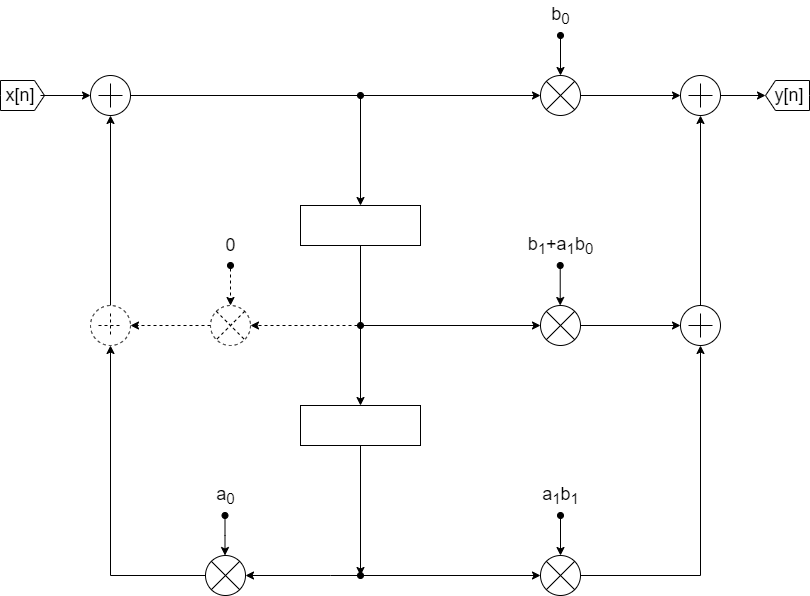
\includegraphics[width=0.7\textwidth]{IIR_2.png}
	\caption{IIR filter with J-look-ahead technique}
	\label{fig:IIR_advanced}
\end{figure}

Questa struttura può essere, al contrario di quella precedente, migliorata in termini di prestazioni. Il percorso critico di questo schema è composto da 4 blocchi combinatori, due moltiplicatori e due sommatori ma attraverso le opportune trasformazioni è possibile ridurre il percorso combinatorio più lungo. In \autoref{fig:IIR_advanced_2} è stato identificato il primo cut-set che permette di spostare il registro modificando la lunghezza del percorso critico portandola da 4 a 3.

\begin{figure}[h]
	\center
	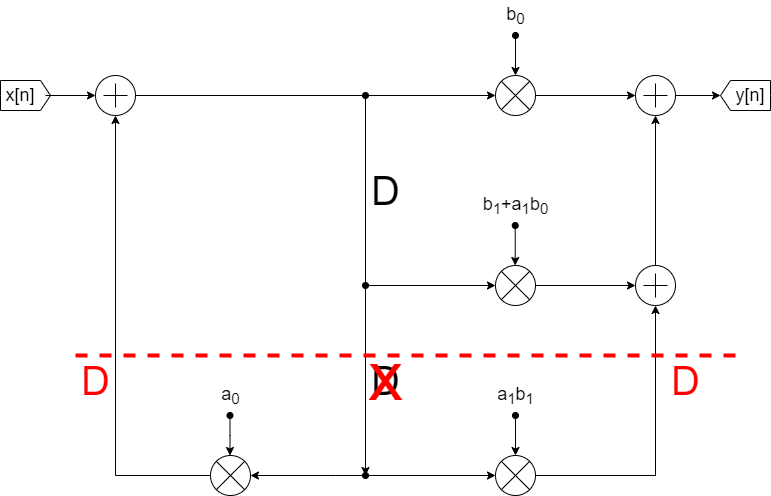
\includegraphics[width=0.7\textwidth]{IIR_2_1.png}
	\caption{Advanced architecture with $1^{st}$ transformation}
	\label{fig:IIR_advanced_2}
\end{figure}

\subsection{Simulation}
Per la simulazione del circuito è stata utilizzato lo stesso testbench precedente in quanto l'entity esterna del cirucito non è cambiata rispetto all'implementazione precedente.
In \autoref{fig:wave_start_j} è mostrato il con i segnali del DUT. In questo caso quando il segnale $VIN$ diventa valido sono necessari 4 colpi di clock prima che il primo risultato sia disponibile in uscita; il motivo di questa latenza più lunga è dato dal tipo diverso di architettura implementata.

\begin{figure}[h]
	\center
	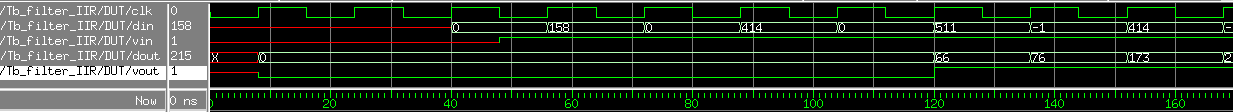
\includegraphics[width=1\textwidth]{images/wave_start_j_look_ahead.png}
	\caption{Start of the simulation}
	\label{fig:wave_start_j}
\end{figure}

Infine in \autoref{fig:wave_vin_j} si nota il correttamento funzionamento del circuito quando $VIN$ diventa basso e successivamente alto. Infatti il segnale $d\_out$ in un primo momento non cambia e da quando il filtro riprende a campionare passano 4 colpi di clock prima di avere i giusti risultati in uscita.

\begin{figure}[h]
	\center
	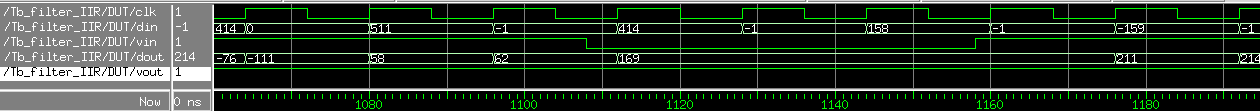
\includegraphics[width=1\textwidth]{images/wave_vin_0_1_j_look_ahead.png}
	\caption{Simulation of the change of $VIN$ signal}
	\label{fig:wave_vin_j}
\end{figure}

Appurato il corretto timing del circuito è stato effettutato il controllo dei dati in uscita confrantondoli conla corrispondente implementazione in C del modello realizzato. A fronte dello stesso set di dati usati per il testbench dell'architettura precedente sono stati ottenuti gli stessi risultati in uscita. Si può fare riferimento ai dati mostrati in \autoref{tab:tab_results} per avere un idea dei risultati.


\subsection{Logic Synthesis}
Verificato il corretto funzionamento del filtro con Modelsim si è passati alla sintesi con Synopsys. Gli obiettivi sonno quelli di cercare la frequenza massima di funzionamento e successivamente impostando $T_{CLK} = 4 T_{min}$ cercare l'area e la potenza consumata, utilizzando i dati sulla switching activity prodotti con Modelsim.
I risultati relativi al periodo di clock, il relativo slack e l'area sono mostrati in \autoref{tab:timing_rep_j}.

\begin{table}[h]
\begin{center}
\begin{tabular}{|l|l|l|}
\hline
$T_{CLK}$ (ns) & slack (ns) & area $(\SI{}{\micro\meter})^2$ \\
\hline
10 & 7.39 &  3200\\
0 & -1.75 &  3834\\
2.15 & 0 & 3542 \\
8.6 & 5.99 & 3200 \\
\hline
\end{tabular}
\end{center}
\caption{Results of timing report}
\label{tab:timing_rep_j}
\end{table}

Successivamente è stata utilizzata netlist generata per calcolare la switiching activity con Modelsim e ottenere in questo modo una stima accurata della potenza consumata dal circuito. I risultati sono mostrati in \autoref{fig:pow_rep_x4_j}.

\begin{figure}[h]
	\center
	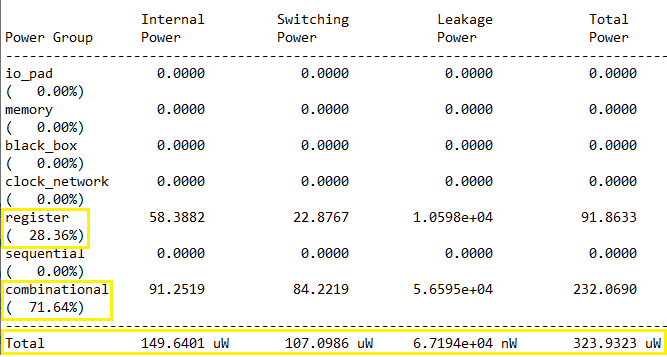
\includegraphics[width=0.8\textwidth]{images/report_power_x4_j_mod.png}
	\caption{Power Report}
	\label{fig:pow_rep_x4_j}
\end{figure}

Anche in questo caso si nota come il consumo di potenza sia dato maggiormente dalla parte combinatoria costituita da N sommatori e M moltilicatori.

\subsection{Place \& Route}
Finally è stato effettutato il placing and routing con il software innovus seguendo la procedura precedente. Il circuito generato è quello mostrato in \autoref{fig:layout_j}, ha un'area pari a $\SI{3186}{\micro\meter}^2$ in accordo con quello ottenuto dal report di Synopsys, con totale di 1588 cells and 3993 gates. I valori ottenuti sono plausibili se rapportati a quelli dell'architettura precedente in quanto in questo caso sono presenti più elementi fisici (registri, sommatori e moltiplicatori) e di conseguenza ci si aspetta la necessità di area maggiore per allocare tutti i gate necessari.

\begin{figure}[h]
	\center
	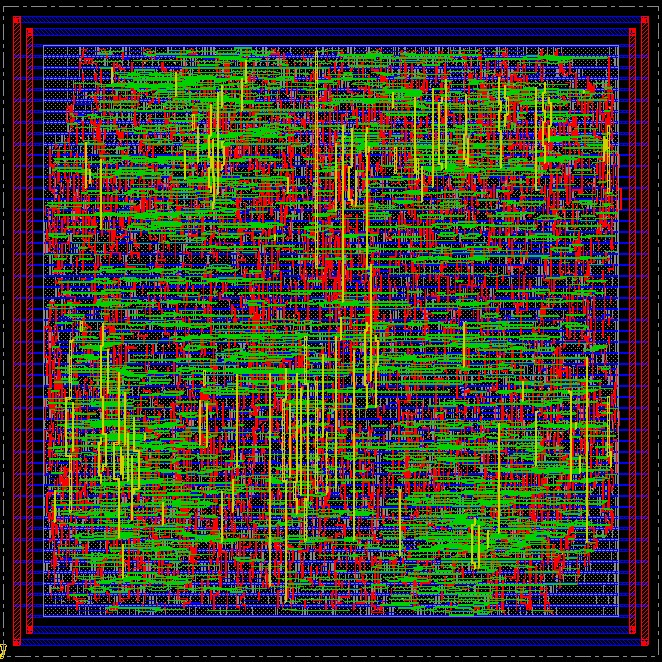
\includegraphics[width=0.6\textwidth]{images/IIR_filter_period_min_x4_place_j.jpg}
	\caption{Resulting layout}
	\label{fig:layout_j}
\end{figure}

Successivamente è stata lancia la timing analysis, la verifica della connectivity e della geometria che hanno evidenziato l'assenza di qualsiasi violazione. Infine è stata un ulteriore stima del consumo di potenza utilizzando la switching activity calcolata con Modelsim. I risultati sono mostrati in \autoref{fig:cadence_pow_rep_x4_j}, anche in questo caso i risultati ottenuti sono in linea con quelli ottenuti dal report di potenza di Synopsys.

\begin{figure}[h]
	\center
	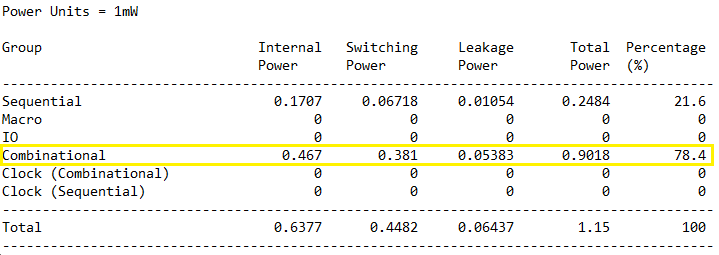
\includegraphics[width=0.8\textwidth]{images/rep_power_x4_cadence_j_mod.png}
	\caption{Post place \& route power report}
	\label{fig:cadence_pow_rep_x4_j}
\end{figure}
